\section{Conclusion}
\SectionPage

\begin{frame}
  \frametitle{Development process}
  \begin{itemize}
    \item Developed using modern development techniques
    \pause
    \begin{center}
      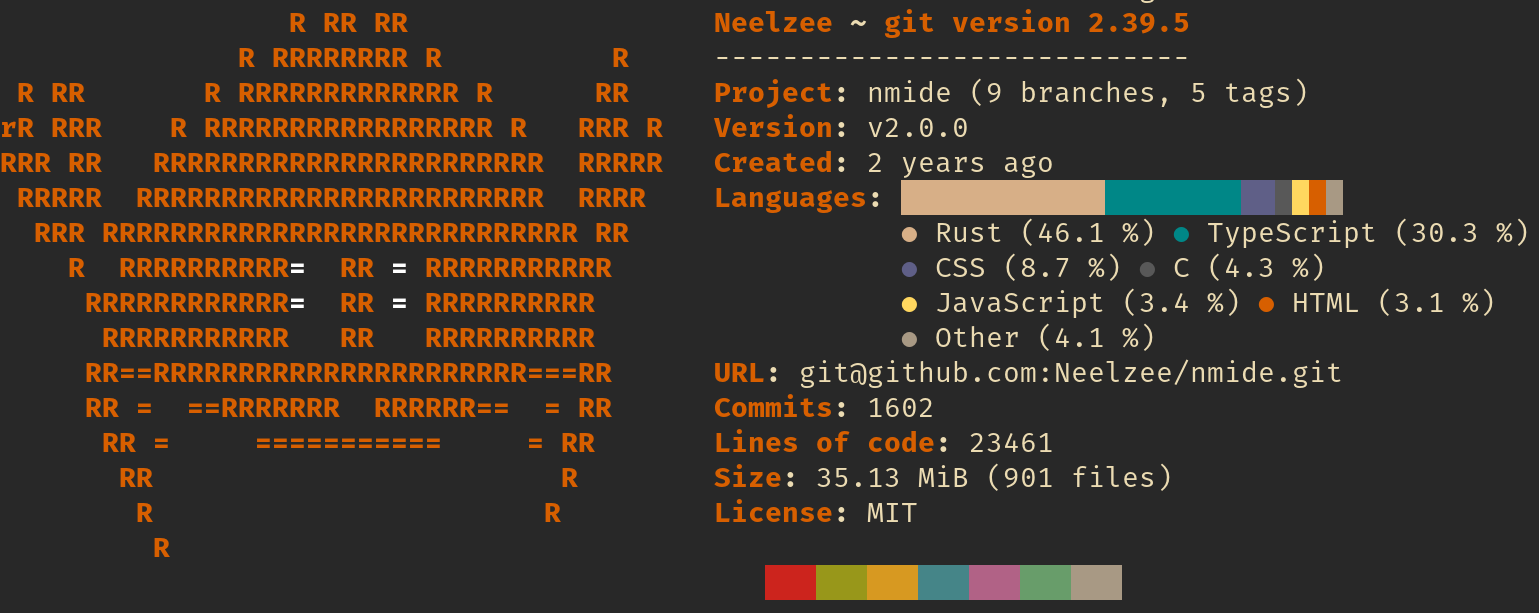
\includegraphics[width=0.8\textwidth]{./pics/onefetch.png}
    \end{center}
  \end{itemize}
\end{frame}

\begin{frame}
  \frametitle{Testing}
  \begin{itemize}
    \item GitHub actions
    \begin{center}
      
\includegraphics[width=0.3\textwidth]{./pics/github-actions.png}
    \end{center}
    \item Tests for the Rust libraries
    \begin{center}
      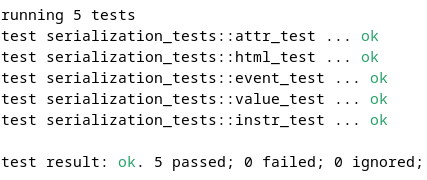
\includegraphics[width=0.45\textwidth]{./pics/librstest.png}
    \end{center}
    \item Tests for the JavaScript libraries
    \begin{center}
      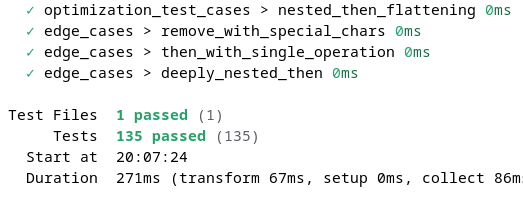
\includegraphics[width=0.45\textwidth]{./pics/libtest.png}
    \end{center}
  \end{itemize}
\end{frame}

\begin{frame}
  \frametitle{Goals}
  \pause
  \begin{itemize}
    \item All functionality comes from modules
    \pause
    \item Modules can be made in different programming languages
    \pause
    \item The core can only load modules
    \pause
    \item Allows for blocking or non-blocking threading
    \pause
    \item The core is modular
    \pause
    \begin{itemize}
      \item Can be run as a web IDE
    \end{itemize}
  \end{itemize}
\end{frame}

\section{Demo}
\SectionPage